\documentclass[%
 reprint,
 amsmath,amssymb,
 aip,
]{revtex4-1}

\usepackage{graphicx}% Include figure files
\usepackage{dcolumn}% Align table columns on decimal point
\usepackage{bm}% bold math
\usepackage{hyperref}% add hypertext capabilities
\usepackage{graphicx}
\usepackage{color}

\preprint{APS/123-QED}
\begin{document}
\title{Acoustics I project: rotating and resonant waves in a cylindrical cavity}
\author{Mathieu Maréchal\\ Supervisor: Guillaume Penelet}
\affiliation{
    M1 Wave Physics \& Acoustics\\Le Mans Université
}%
\date{\today}

\begin{abstract}
    \textbf{Abstract:} abstract abstract abstract abstract abstract abstract abstract abstract abstract abstract abstract abstract abstract abstract abstract abstract abstract abstract abstract abstract abstract abstract abstract abstract abstract abstract abstract abstract abstract abstract abstract abstract abstract abstract abstract abstract abstract abstract abstract abstract abstract abstract abstract abstract abstract abstract abstract abstract abstract abstract abstract abstract abstract abstract abstract abstract abstract abstract abstract abstract abstract abstract abstract abstract abstract.
\end{abstract}

\maketitle
\section{Introduction}
Cylindrical waveguides and modal analysis are among the key notions tackled in the Acoustics I class. And what better way to make use of these two notions than to study rotating waves. This present paper describes the project led within the framework of this course, dealing with resonant and rotating waves in a cylindrical resonant cavity. Rotating waves are not a very hot topoc within the acoustics research topics, they are more dealt with for quantum and electromagnetic waves. However, they were studied by Ceperley \cite{ceperley2002} who introduces rotating waves for water and for acoustics. One interesting aspect to this type of wave is that it transfers its angular momentum to matter as studied by \emph{Santillan et al.} \cite{santillan2009}. What follows will focus on the ways to generate an acoustic vortex or in other words, a rotating wave field. This study will be done in several parts. Firstly, one has to study analytically the characteristics of the considered cylindrical cavity, and in particular its nodal lines for specific modes, along which the point sources generating the rotating field will be placed. Then, making use of the superposition principle, one will be able to numerically simulate several phase-shifted sources exciting the cavity. Finally, controlling the phasing of these sources, one should be able to control the nature of the wave propagating in the cavity, thus allowing the production of a vortical wave field. 

\section{Derivation of the pressure field inside the cylinder using modal analysis}
The system considered in this paper is a cylinder which includes one (and thereafter several) loudspeaker seen as a point source located at $\vec{r}_0 = (r_0, \theta_0, z_0)$ creating an acoustic field $\tilde{p}(\vec{r}, t)$, $\vec{r} = (r, \theta, z)$. This point source imposes a driving force $q_0$ oscillating at a $\omega$ frequency. The cylinder is filled with air, a lossless medium with density $\rho_0 = 1.2$ kg.m$^3$ and sound celerity $c_0 = 343$ m/s. Its radius is denoted $R$ and its length as $d$. A representation of the studied system is proposed in figure \ref{fig:schema}.

\subsection{Modal expansion in the two-dimensional case}
During this part, a 2D pressure field $\tilde{p}(r, \theta)$ will be considered: it will only depend on its azimuthal $\theta$ and radial $r$ coordinates, and we will write that $d \ll R$. The wave equation to solve in the cavity is inhomogenenous,
\begin{equation}
    \begin{split}
        \frac{\partial \tilde{p}^2}{\partial r^2} + \frac{1}{r} \frac{\partial \tilde{p}}{\partial r} &+ \frac{1}{r^2} \frac{\partial \tilde{p}^2}{\partial \theta^2} + k^2 \tilde{p}\\ &= -i \omega q_0 \delta(r - r_0) \delta(\theta - \theta_0),
    \end{split} \label{eq:2dwaveq}
\end{equation}
with $k = \omega/c_0$ being the wavenumber and $\delta$ is the Dirac-Delta distribution.
The edges of the cavity are all considered rigid, thus giving the following boundary conditions on the acoustic field
\begin{equation}
   \begin{split}
       \tilde{p}(r, \theta + 2 \pi , z) &= \tilde{p}(r, \theta, z),\\
               \left. \tilde{v}_r \right|_{r=R} & = 0 \Rightarrow J'_m (k_{mn}R) = 0.
   \end{split} \label{eq:bc2d}
\end{equation}
Due to the periodicity condition, we have that the clockwise and anticlockwise spinning modes $m \in \mathbb{Z}$ are integers. Furthermore, due to the Bessel functions properties stating that $J_m = (-1)^m J_{-m}$ the same order symmetric modes $m$ and $-m$ are eigenpairs and share the same eigenvalues \cite{rona2007}, so that $m \in \mathbb{N}$.

The solution of the field can be written by making use of modal analysis method, which tells us that any pressure field can be generally written as 
\begin{equation}
    \tilde{p}(r, \theta) = \sum_{m,n} \tilde{C}_{mn} \Psi_{mn}.
\end{equation}
Where $\tilde{C}_{mn}$ is a term representing the amplitude of the field, and $\Psi_{mn}$ is the eigenfunctions, determined using the boundary conditions from equation (\ref{eq:bc2d}). Using $\Psi_{mn} = \tilde{C}_{mn} J_m (k_{mn}r)\left[ \tilde{A}_{\theta m} \cos(m \theta) + \tilde{B}_{\theta m} \sin(m \theta) \right]$ as set of eigenfunctions, we will be able to find the amplitude expression. To do that, one has to orthogonalize or normalize each part of the eigenfunction.

First of all, in order to make calculations a bit simpler, the eigenfunction can be rewritten as
\begin{equation}
        \tilde{p}(r, \theta) = \sum_{mn}^{\infty} J_m(k_{mn}r) \left[ \tilde{A}_{mn} \cos(m \theta) + \tilde{B}_{mn} \sin(m \theta) \right], \label{eq:gensol}
\end{equation}
where the amplitude term $\tilde{C}_{mn}$ can be expressed inside $\tilde{A}_{\theta_{mn}}$ and $\tilde{B}_{\theta_{mn}}$, which were thus respectively renamed $\tilde{A}_{mn}$ and $\tilde{B}_{mn}$. 

Subsequently, the pressure field written in equation (\ref{eq:gensol}) can be put in equation (\ref{eq:2dwaveq}), which leads to
\begin{equation}
    \begin{split}
        \sum_{mn} &\left[ k^2 - k_{mn}^2 \right] J_m(k_{mn}r) \Big[ \tilde{A}_{mn} \cos(m\theta) \\&+ \tilde{B}_{mn} \sin(m\theta) \Big]= - i \omega_0 q_0 \delta(r - r_0) \delta(\theta - \theta_0)
    \end{split} \label{eq:rawsol}
\end{equation}

\begin{figure}
    \centering
    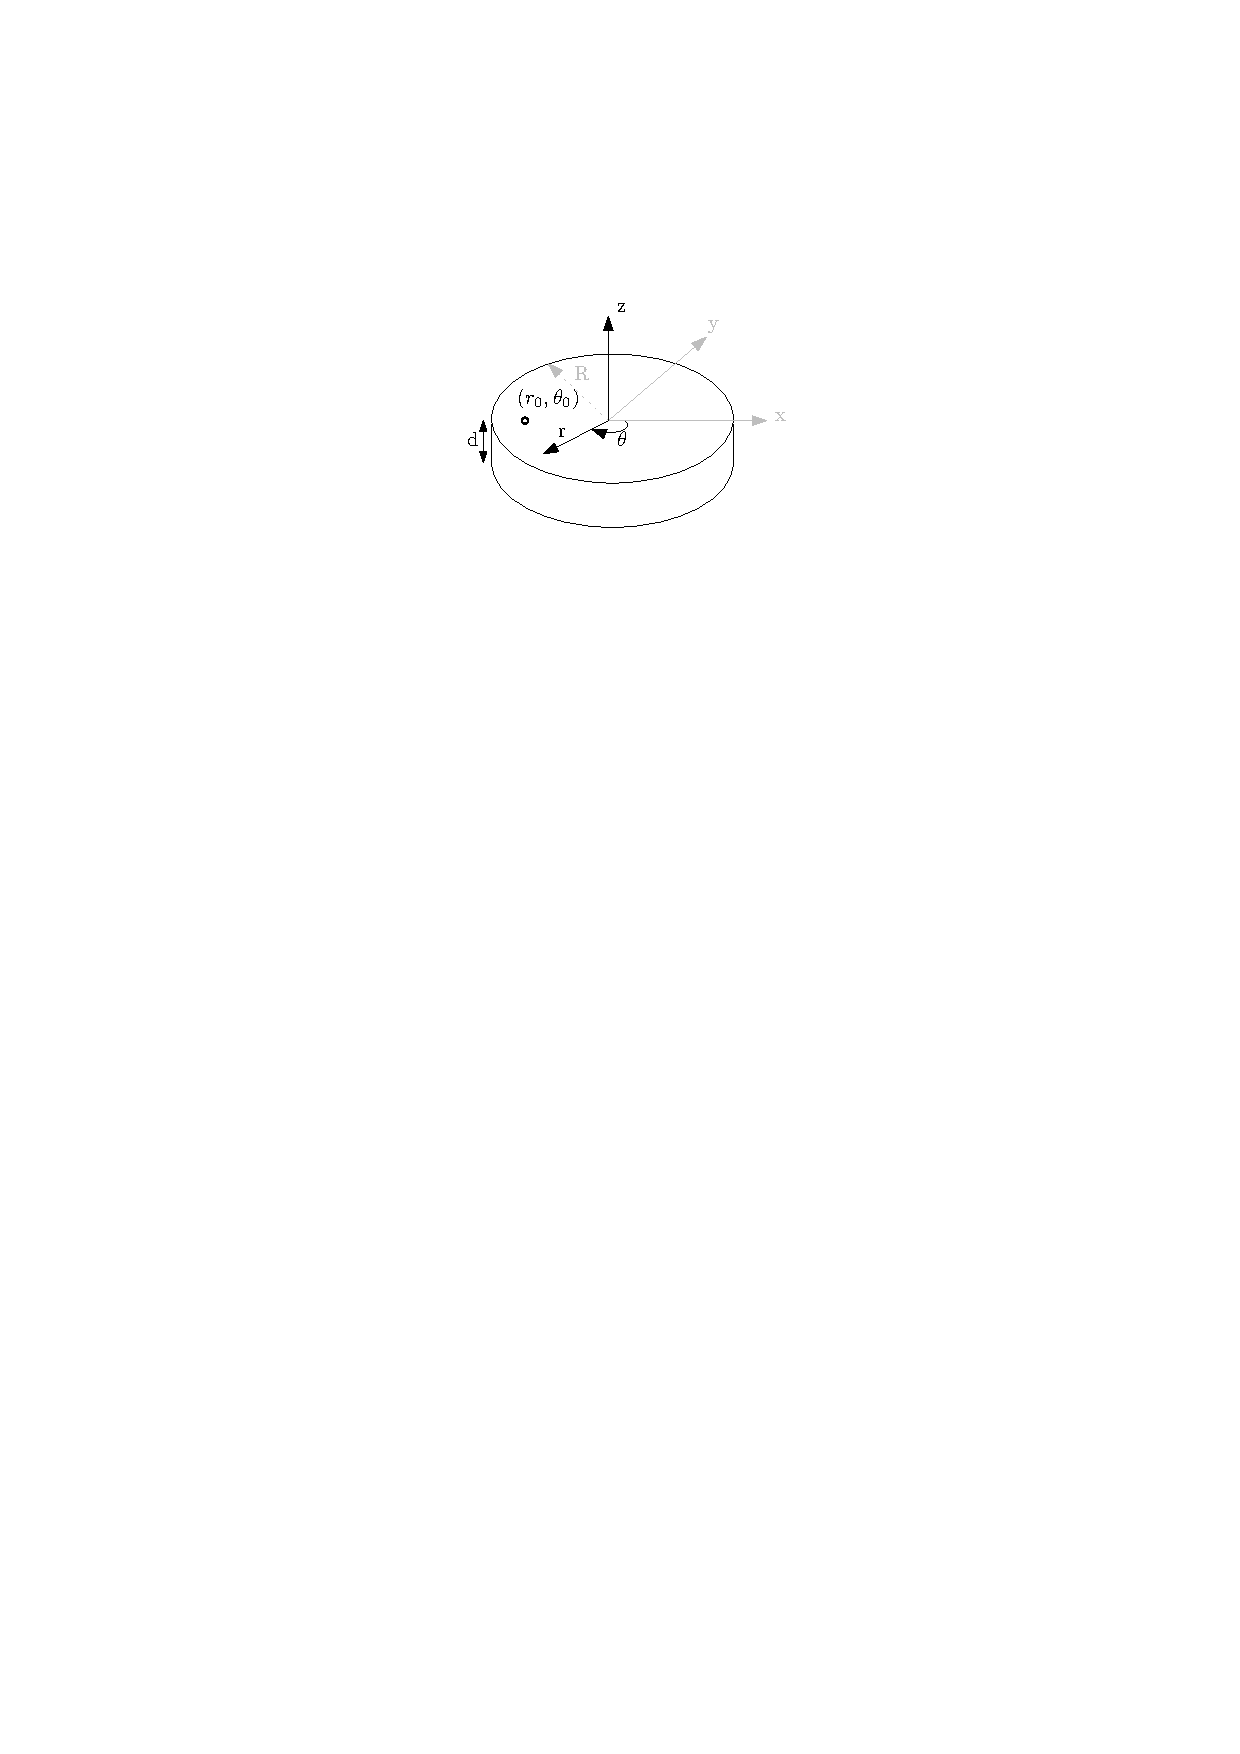
\includegraphics[width=.35\textwidth]{figures/schema.pdf}
    \caption{Representation of the cylindrical cavity of radius $R$ and height $d$ with one point source at $(r_0, \theta_0)$}
    \label{fig:schema}
\end{figure}

Now to the orthogonalization part: we will here proceed to normalize each part of the eigenfunction using the following integral results
\begin{equation}
   \int_0^{2 \pi} \cos^2\left( m \theta \right) d\theta = 
    \begin{cases}    
        2 \pi, & m = 0\\
        \pi, & m \ne 0
    \end{cases}, \label{eq:dp_2}
\end{equation}

\begin{equation}
    \int_0^{2 \pi} \sin^2\left( m \theta \right) d\theta = 
    \begin{cases}    
        0, & m = 0\\
        \pi, & m \ne 0
    \end{cases}, \label{eq:dp_3}
\end{equation}
and one property of the Bessel function is
\begin{equation}
    \begin{split}
        \int_0^{R} &r J^2_m (k_{mn} r)dr \\ &=
    \begin{cases}    
        \quad  \quad \quad 1/2, & k_{mn}R = 0\\
        \frac{k^2_{mn} R^2 - m^2}{2 k^2_{mn}} J^2_m (k_{mn} R), & k_{mn}R \ne 0
    \end{cases}.
    \end{split} \label{eq:dp_4}
\end{equation}

These results can be used in our calculations. Therefore, they can be rewritten in a more aesthetic way using the Kronecker delta symbol defined as 
\begin{equation}
   \delta_i^j = \begin{cases}
       1, & i = j\\ 0, & i \ne j
   \end{cases} 
\end{equation}

That way, equations (\ref{eq:dp_2}) and (\ref{eq:dp_3}) are respectively equal to $\pi(1 + \delta_m^0)$ and $\pi(1 - \delta_m^0)$. Finally, the case for $k_{mn}R = 0$ in equation (\ref{eq:dp_4}) can be discarded as it is a solution that is trivial (nothing is happening in the cavity).

These operations can be also simply described as an integration over the surface of the studied disk, and multiplying equation (\ref{eq:rawsol}) by successively $r J_m(k_{mn}r) \cos(m\theta)$ in order to retrieve $\tilde{A}_{mn}$ and $r J_m(k_{mn}r) \sin(m\theta)$ to get $\tilde{B}_{mn}$. After the application of these operations, we end up with
\begin{equation}
    \begin{split}
        \tilde{A}_{mn} =& \frac{- 2 i \omega_0 q_0 r_0}{\pi (1 + \delta_m^0)} k_{mn}^2  \cos(m \theta_0) \frac{J_m(k_{mn}r_0)}{J^2_m(k_{mn}R)}\\ &\times\left[(k^2 - k^2_{mn}) ((k_{mn}R)^2 - m^2)\right]^{-1}
    \end{split}
\end{equation}
and 
\begin{equation}
    \begin{split}
        \tilde{B}_{mn} =& \frac{- 2 i \omega_0 q_0 r_0}{\pi (1 - \delta_m^0)} k_{mn}^2  \sin(m \theta_0) \frac{J_m(k_{mn}r_0)}{J^2_m(k_{mn}R)}\\ &\times\left[(k^2 - k^2_{mn}) ((k_{mn}R)^2 - m^2)\right]^{-1}
    \end{split}
\end{equation}

The expression for the two amplitude terms can be used in equation \ref{eq:gensol} and the pressure field of a point source can be calculated. This will be implemented in a Python script which will allow us to visualise the mode shapes of the cylindrical cavity.  

\section{Resonant modes of the cavity and influence of the point source parameters on the resonances}
\subsection{Investigation with one source}
Now that the pressure field expression was derived, one can make use of this analytical solution to plot the resonance modes of the cylindrical cavity. A figure can be constituted for a range of modes $mn$ from 10 to 22, and is presented in figure \ref{fig:modes}. The mode shapes are quite close to the fundamental patterns given by $J_m(k_{mn})\cos(m\theta)$ (as represented in the lecture notes). However, the position of the source has an influence on the pressure distribution along the disk: the nodes closer to the source are more excited than the other. What is more is that, the excitation frequency of the source is not strictly the same as a given mode resonance frequency due to the term $\left.\left[k^2 - k^2_{mn}\right]^{-1}\right|_{k = k_{mn}} \longrightarrow \infty$. This doesn't do good with computer simulations, so we restrain ourselves with a close-enough value for $k \approx k_{mn}$ in order to mostly excite the mode we want to observe.

\begin{figure}
    \centering
    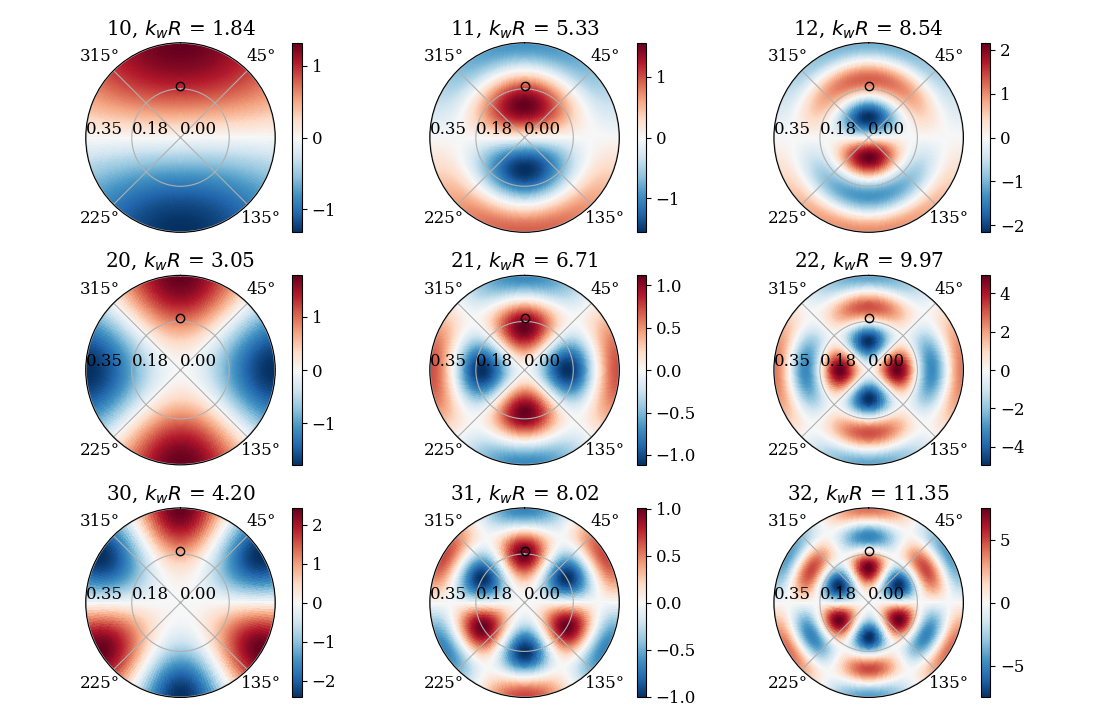
\includegraphics[width=.5\textwidth]{figures/modes.png}
    \caption{Modes $mn$ of the cavity generated by a single point source, represented by a black hollow circle and located at ($r_0$ = $R/2$, $\theta_0$ = $\pi$), emitting a flow $q_0 = 10^{-2}$ m$^3$/s with a frequency close to the resonance of each mode $\omega_0 = c_0 \: (k_{mn} + 0.1)$. The real pressure field is normalized with respect to the pressure at the point source.}
    \label{fig:modes}
\end{figure}

An important part of the simulations is the positioning of the source inside the cavity, which we need to understand if we want to generate rotating waves. 

\begin{figure}
    \centering
    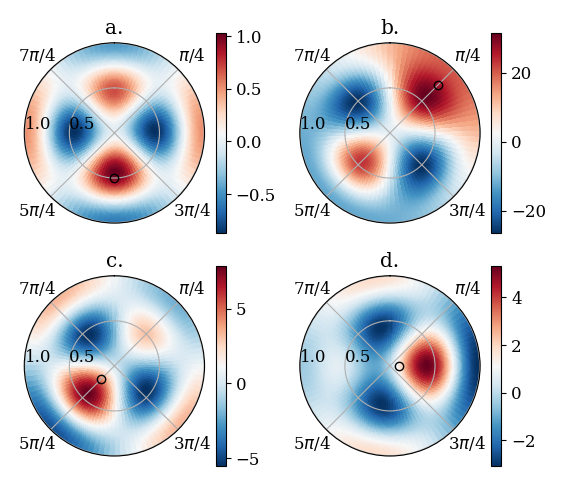
\includegraphics[width=.5\textwidth]{figures/source_pos.png}
    \caption{Pressure distribution in the cavity for different source positions. The source in all cases emits a flow $q_0 = 10^{-2}$ m$^3$/s with a frequency $\omega_0 = c_0 \: (k_{mn} + 5\%)$. The position for each subfigure are: a. $(0.5, \pi)$, b. $(0.75, \pi/4)$, c. $(0.2, 5 \pi/4)$, d. $(0.1, \pi/2)$.}
    \label{fig:source_pos}
\end{figure}

\subsection{Adding more sources in the cavity}
Add sources whose behaviour is governed by the same equations as before. Make use of the superposition principle. plot the thing. 

\section{Simulating rotating waves in the cavity}
One way of studying and trying to observe rotational waves would be to put our considered sources along nodal lines: if one uses for example the nodal lines for the 11 mode, it's quite easy as one nodal line has a circular shape along the cylinder edge, at around $r = 0.25$ m.
\begin{figure}
   \centering 
   \def\svgwidth{0.5\textwidth}
   \input{contour_time.pdf_tex}
   %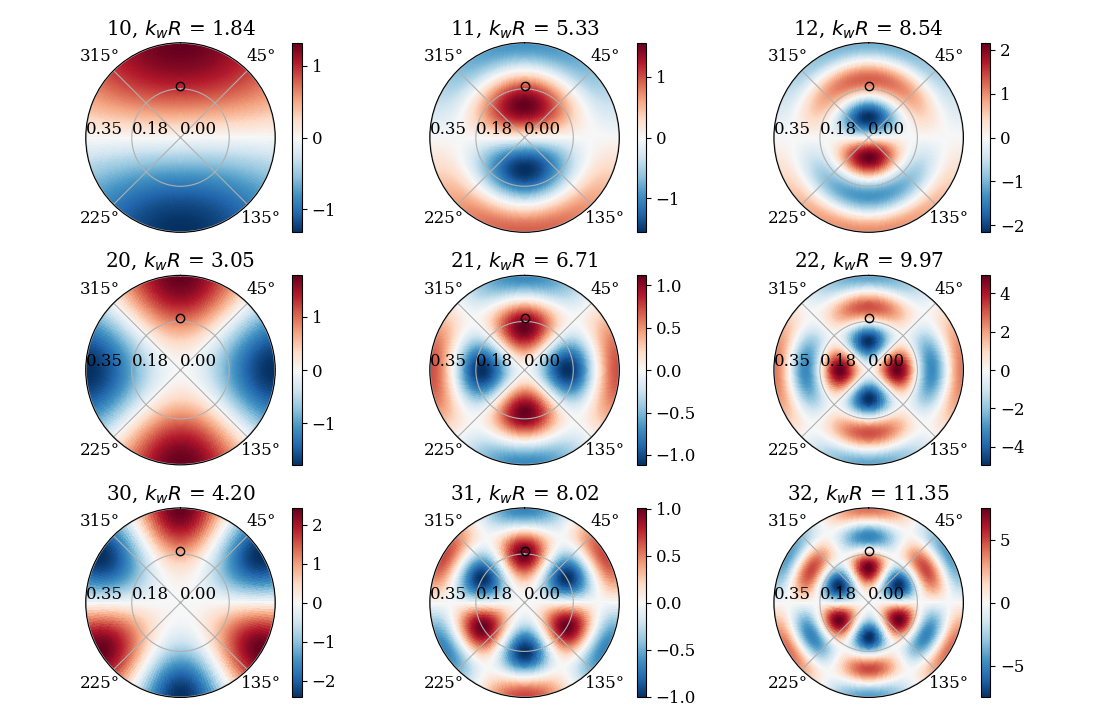
\includegraphics[width=.5\textwidth]{figures/modes.png}
   \caption{Rotation of waves inside the cavity with 4 sources emitting an acoustic wave with each its own phasing. The mode 10 of the cavity is excited and the waves rotates in the clockwise direction} 
   \label{eq:contour_time}
\end{figure}

yeys

\section{Extension of the study to 3D}
In order to extend the previous equations to the three dimensional case, the first thing to do is that one has to add a boundary condition at $z=0$ and $z=d$.
\begin{equation}
   \left. \tilde{v}_z \right|_{z=0} = \left. \tilde{v}_z \right|_{z=d} = 0,
\end{equation}
The wavenumber is now
\begin{equation}
    k^2 = k_{mn}^2 + k_z^2,
\end{equation}
with $k_z = \frac{l \pi}{d}$

Need to make use of the previous integral results add one more
\begin{equation}
    \int_0^l \cos^2\left( \frac{l \pi}{d}z \right) dz = 
    \begin{cases}    
        d, & l = 0\\
        d/2, & l \ne 0
    \end{cases} \label{eq:dp_1}
\end{equation}
Similarly, this can be rewritten as $\cfrac{d}{2 - \delta_l^0}$.

The pressure field is
\begin{equation}
    \begin{split}
        \tilde{p}(r, \theta, z) &= \sum_m^{\infty}\sum_n^{\infty}\sum_l^{\infty} J_m(k_{mn}r) \cos(k_z z)\\ &\times \left[ \tilde{A}_{mnl} \cos(m \theta) + \tilde{B}_{mnl} \sin(m \theta) \right],
    \end{split}
\end{equation}

The solution for the amplitude terms can be written as 
\begin{equation}
    \begin{split}
        \tilde{A}_{mnl} = &\frac{2 q^{\star} r_0 k^2_{mn} \cos(k_z z_0) \cos(m \theta_0)}{\pi d\left[k^2 - k^2_{mn}\right] \left[(k_{mn}R)^2 - m^2 \right]}\\  &\times \frac{2 - \delta_l^0}{1 + \delta_m^0} \frac{J_m(k_{mn}r_0)}{J^2_{m}(k_{mn}R)},
    \end{split}
\end{equation}
and
\begin{equation}
    \begin{split}
        \tilde{B}_{mnl} = &\frac{2 q^{\star} r_0 k^2_{mn} \cos(k_z z_0) \sin(m \theta_0)}{\pi d\left[k^2 - k^2_{mn}\right] \left[(k_{mn}R)^2 - m^2 \right]}\\  &\times \frac{2 - \delta_l^0}{1 - \delta_m^0} \frac{J_m(k_{mn}r_0)}{J^2_{m}(k_{mn}R)}.
    \end{split}
\end{equation}

\section{Perspectives on this short study}
- FEM simulation
- experimental setup
- understand the phenomenon more, to get how to produce pure rotating waves --> introduce something like the standing wave ratio but for rotating ?
- all kinds of things

\section{Conclusion}
One perspective from this study is that an experimental study could follow from the results obtained above. A simple apparatus can be developed and some experimental data could be compared to the theoretical and numerical study that was conducted here. Every content of this project including the scripts is available on Github: \url{https://github.com/marecmat/VorticalWavesAcoustics}

\bibliography{biblio}



\end{document}

Finally, the equation for the pressure field is 
\begin{equation}
    \begin{split}
        \tilde{p}(r, \theta) = &\frac{2i \omega q_0 r_0}{R^2}\bigg[ \frac{1}{k^2} + \sum_{m=1, n}^{\infty} \frac{2}{k_{mn}^2-k^2} \frac{J_m(k_{mn} r_0)}{J^2_m(k_{mn} R)}\\ & \times \left(1 - \frac{m^2}{k^2_{mn} R^2}\right)^{-1} J_m (k_{mn}r)\cos(m\theta) \bigg] .
    \end{split}
\end{equation}

